\chapter{Graf przetwarzania sygnałów} \label{dsp_graph_chapter}

Na potrzeby badań zostało zaimplementowane środowisko, pozwalające na dynamiczne tworzenie grafów przetwarzania
sygnałów~(\ref{fig:example_simple_analog_synth}). W projekcie nie zostało zastosowane gotowe rozwiązanie symulujące syntezator modułowy, takie jak
\href{https://www.bespokesynth.com/}{Bespoke Synth}~\cite{bespoke}, \href{https://vcvrack.com/Rack}{VCVRack}~\cite{vcvrack}
lub \href{https://puredata.info/}{Pure Data}~\cite{pure_data}, ponieważ
nie udostępniały one gotowego interfejsu pozwalającego na łatwą integrację z językiem \texttt{Python}.
Istniejące w internecie gotowe przykłady algorytmów syntezy audio pozwoliły na szybkie zaimplementowanie
środowiska eksperymentowego, które posiada szeroki zbiór dostępnych algorytmów DSP oraz w przystępny sposób
interfejsuje się z językiem \texttt{Python}, co umożliwia wykorzystanie gotowych pakietów obliczeniowych z dziedziny przetwarzania sygnałów.

\begin{figure}[H]
    \centering
    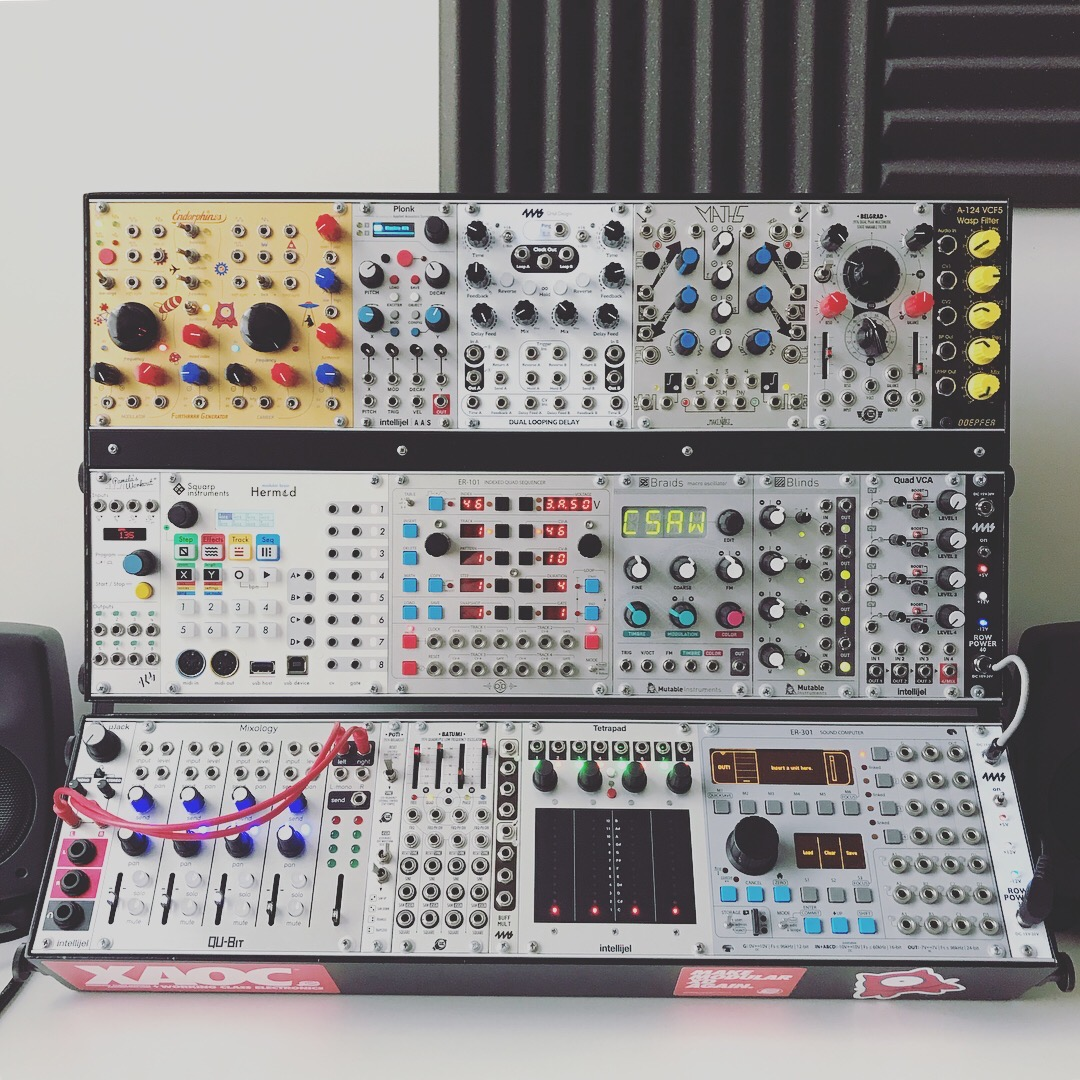
\includegraphics[width=0.4\linewidth]{rys02/eurorack.jpg}
    \caption{
      Przykładowy układ modułów w standardzie \textit{Eurorack}~\cite{eurorack}.
      W prawym dolnym rogu widoczne połączenia modulujące między modułami.
    }
    \label{fig:eurorack_setup}
\end{figure}

\section{Podstawy syntezy dźwięku w syntezatorach modułowych}

Proces syntezy dźwięku może zostać przedstawiony jako zbiór węzłów wykonujących syntezę lub
przetwarzanie sygnału audio oraz połączeń między węzłami. Przykładowe elementy grafu:

\begin{enumerate}
  \item Węzły:
    \begin{enumerate}
      \item generujące sygnał:
        \begin{itemize}
          \item synteza sygnałów (sinusoida, trójkąt, sygnał prostokątny),
          \item sygnał modulujący (LFO, ADSR).
        \end{itemize}
      \item przetwarzające sygnał:
        \begin{itemize}
          \item filtry (górnoprzepustowy, dolnoprzepustowy, pasmowo-przepustowy),
          \item efekty (pogłos, echo).
        \end{itemize}
    \end{enumerate}
  \item Połączenia między węzłami:
    \begin{itemize}
      \item modulowanie parametrów syntezy i przetwarzania sygnału.
    \end{itemize}
\end{enumerate}

\noindent
Odpowiednikiem implementowanego środowiska w świecie rzeczywistym są syntezatory modułowe (przykładowo~\ref{fig:eurorack_setup}),
które pozwalają na dowolne łączenie modułów wykonujących operacje DSP.
Barwę dźwięku w syntezatorze modyfikuje się na dwa sposoby:
\begin{enumerate}
  \item Ustawienie stałej wartości danego parametru w węźle DSP,
  \item Modulacja wartości danego parametru w węźle DSP za pomocą wartości wyjściowej innego węzła.
\end{enumerate}

\begin{figure}[H]
    \centering
    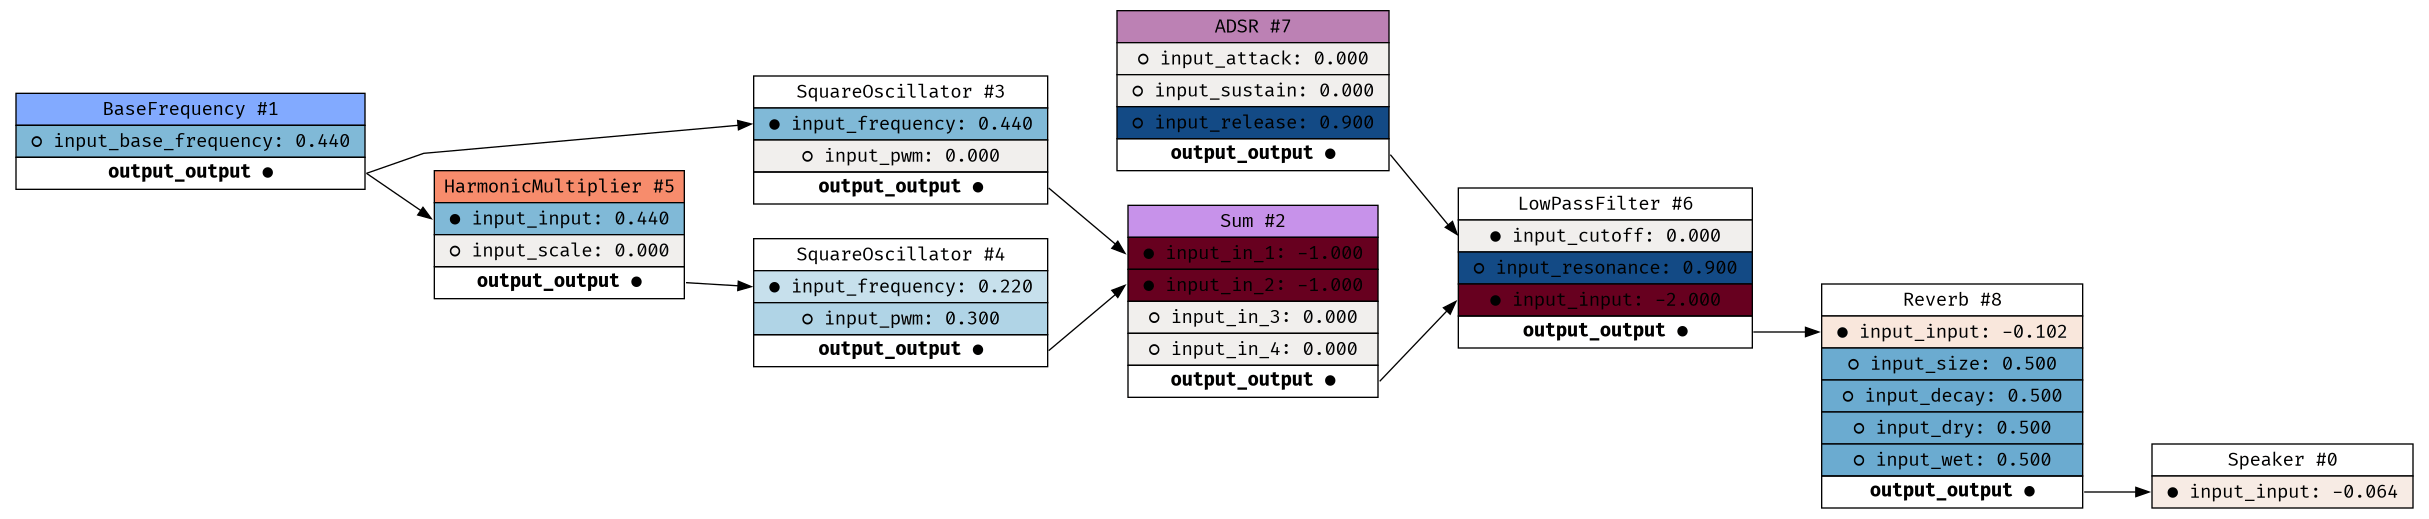
\includegraphics[width=0.9\linewidth]{rys02/luthier_simple_analog.png}
    \caption{
      Przykładowy układ węzłów DSP w zaimplementowanym środowisku eksperymentowym.
      Układ wykonuje syntezę subtraktywną z modulowaną wartością częstotliwości granicznej filtru niskoprzepustowego
      oraz dodaje efekt pogłosu (\textit{reverb})~\cite{reverb}.
    }
    \label{fig:example_simple_analog_synth}
\end{figure}

\noindent
Dla przykładowego układu DSP, przedstawionego na rysunku~\ref{fig:example_simple_analog_synth},
skonfigurowane są między innymi parametry:

\begin{enumerate}
  \item Częstotliwość podstawowa (węzeł \texttt{BaseFrequency \#1}),
  \item wartość, przez którą mnożona jest częstotliwość podstawowa w węźle \texttt{HarmonicMultiplier \#5},
  \item Wartości \texttt{input\_pwm} w węzłach \texttt{SquareOscillator} \texttt{\#3} oraz \texttt{\#4},
  \item Parametry algorytmu pogłosu w węźle \texttt{Reverb \#8}.
\end{enumerate}

\noindent
Z kolei wartość parametru \texttt{input\_cutoff} w węźle \texttt{LowPassFilter \#6} \textbf{jest modulowana}
przez sygnał wychodzący w węźle \texttt{ADSR \#7}, co pozwala na dynamiczne zmiany
częstotliwości odcięcia filtru w czasie, wzbogacając barwę generowanego dźwięku.

\section{Wymagania} \label{sec:requirements}

W ramach pracy zostały zdefiniowane wymagania dotyczące implementowanego później środowiska eksperymentowego,
opisane w niniejszym rozdziale.

\subsection{Węzły DSP}

Pojedynczy węzeł DSP może zostać opisany za pomocą trzech cech:

\begin{enumerate}
  \item Zbiór sygnałów wejściowych,
  \item zbiór sygnałów wyjściowych,
  \item wykonywana przez węzeł operacja.
\end{enumerate}


% \begin{multicols}{2}
\begin{figure}[H]
    \centering
    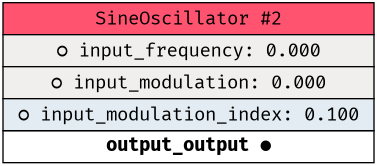
\includegraphics[width=0.4\linewidth]{rys02/example_sine_node.png}
    \caption{
      Węzeł DSP w zaimplementowanym środowisku eksperymentowym, generujący falę sinusoidalną z możliwością modulacji fazy.
    }
    \label{fig:example_sine_node}
\end{figure}

\begin{figure}[H]
    \centering
    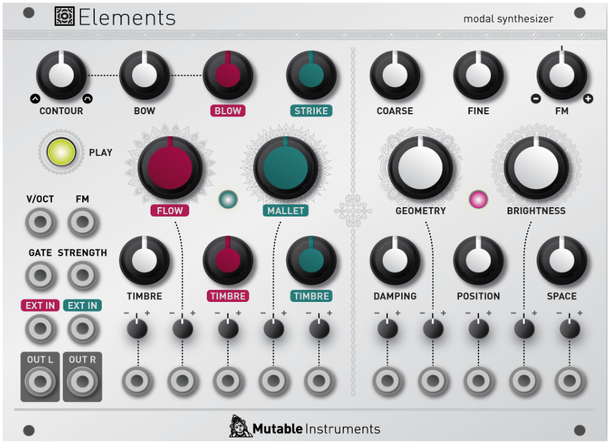
\includegraphics[width=0.45\linewidth]{rys02/mutable_instruments_elements.png}
    \caption{
      Moduł syntezy \textit{Mutable Instruments Elements}, umożliwiający ręczne ustawianie \textbf{oraz} modulację
      parametrów. Moduł wykonuję syntezę typu \textit{physical modeling} \cite{lisp_synthesis}.
    }
    \label{fig:example_eurorack_module}
\end{figure}
% \end{multicols}

\noindent
Przykładowo, przedstawiony na rysunku~\ref{fig:example_sine_node} węzeł posiada:
\begin{enumerate}
  \item sygnały wejściowe:
  \begin{itemize}
    \item \texttt{input\_frequency} - częstotliwość generowanej sinusoidy,
    \item \texttt{input\_modulation} - wartość modulacji fazy, według równania~\ref{eq:fm_sine},
    \item \texttt{input\_modulation\_index}.
  \end{itemize}
  \item Sygnały wyjściowe:
  \begin{itemize}
    \item \texttt{output\_output} - wartość generowanego sygnału sinusoidalnego.
  \end{itemize}
\end{enumerate}

\noindent
Węzeł generuje sygnał sinusoidalny o fazie modulowanej poprzez parametr \texttt{input\_modulation} z siłą modulacji ustawianą przez
parametr \texttt{input\_modulation\_index}, opisane za pomocą równania~\ref{eq:fm_sine}
(jest to uproszczenie równania syntezy FM przedstawionego w \cite{spectral_audio_processing}) oraz listingu~\ref{lst:sine_fm}:

\begin{equation} \label{eq:fm_sine}
  f(t) = sin(t * f + m * m_i)
\end{equation}

\begin{lstlisting}[language=Rust, caption=Implementacja węzła SineOscillator.,label={lst:sine_fm}]
impl DspNode for SineOscillator {
    fn tick(&mut self) {
        let frequency = (self.input_frequency * 1000.0).abs();
        let phase_diff = (2.0 * std::f64::consts::PI * frequency) / SAMPLE_RATE;
        self.output_output =
            (self.phase + self.input_modulation * self.input_modulation_index * 10.0).sin();
        self.phase += phase_diff;

        while self.phase > std::f64::consts::PI * 2.0 {
            self.phase -= std::f64::consts::PI * 2.0
        }
    }
}
\end{lstlisting}

\noindent
\textbf{Wymaganie:} zaimplementowane w ramach pracy środowisko eksperymentalne musi pozwalać na zdefiniowanie węzłów DSP, które generują lub
przetwarzają sygnał. Węzły posiadają sloty wejściowe, z których czytają wartości parametrów sterujących wykonywanymi 
przez węzły operacjami.

\subsection{Połączenia między węzłami -- modulacja parametrów węzłów} \label{sec:modulation_requirements}

Każdy węzeł DSP w środowisku eksperymentowym posiada zbiór parametrów wejściowych. Poza możliwością
ustawienia danego parametru wejściowego na konkretną wartość, możliwa jest też modulacja parametru
wejściowego. Na rysunku~\ref{fig:fm_mod_example} przedstawiony jest przykładowy układ węzłów i modulacji,
które pozwalają na uzyskanie syntezy FM.

\begin{figure}[H]
    \centering
    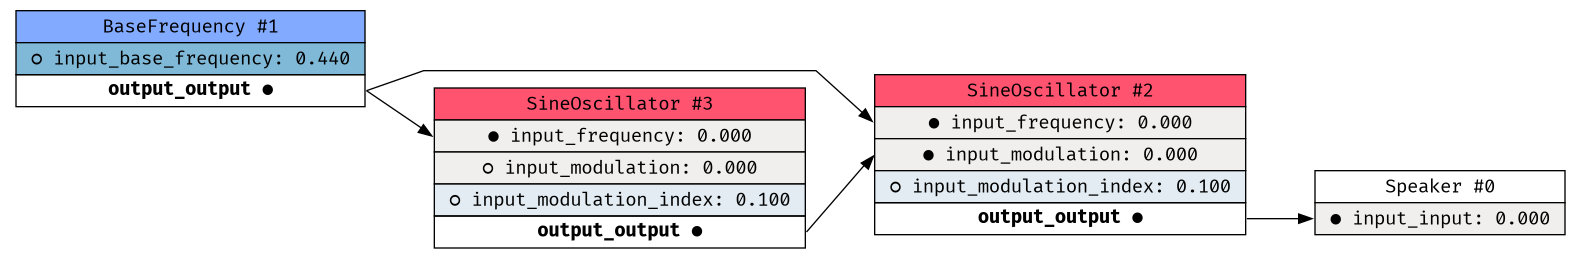
\includegraphics[width=1.0\linewidth]{rys02/fm_mod_example.png}
    \caption{
      Przykładowa modulacja parametru \texttt{input\_modulation} za pomocy sygnału sinusoidalnego, charakterystyczna dla syntezy typu FM \cite{computational_music_synthesis}.
    }
    \label{fig:fm_mod_example}
\end{figure}

\begin{multicols}{2}
\begin{figure}[H]
    \centering
    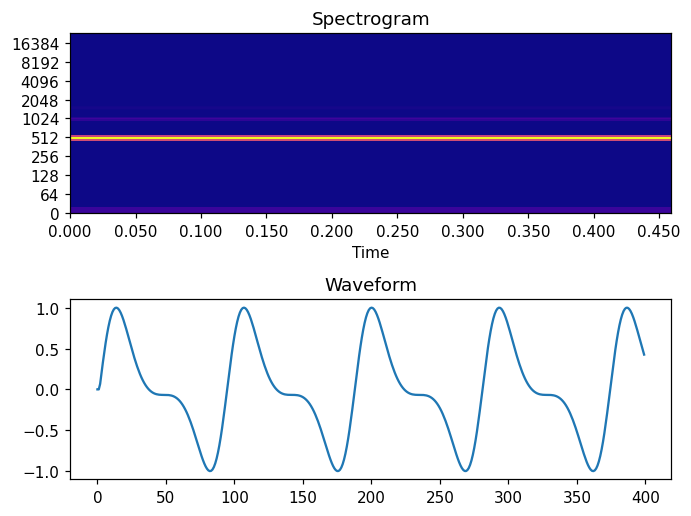
\includegraphics[width=1.0\linewidth]{rys02/spectro_fm.png}
    \caption{
      Spektrogram oraz wykres sygnału wygenerowanego za pomocą układ z rysunku~\ref{fig:fm_mod_example}.
      Widoczne dodatkowe składowe harmoniczne wpływające na barwę dźwięku.
    }
    \label{fig:fm_mod_spectra}
\end{figure}

\begin{figure}[H]
    \centering
    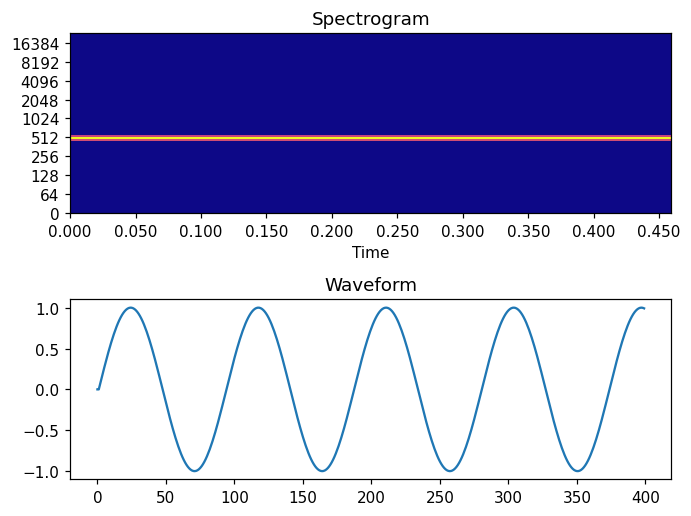
\includegraphics[width=1.0\linewidth]{rys02/spectro_no_fm.png}
    \caption{
      Spektrogram oraz wykres sygnału wygenerowanego przez układ z rysunku~\ref{fig:fm_mod_example}
      \textbf{po usunięciu} połączenia modulującego fazę oscylatora \texttt{\#2}.
      Widoczna tylko jedna składowa harmoniczna: częstotliwość podstawowa.
    }
    \label{fig:fm_no_mod_spectra}
\end{figure}
\end{multicols}

\noindent
\textbf{Wymaganie:} zaimplementowane środowisko pozwala na modulowanie
dowolnego parametu wejściowego w węźle za pomocą wartości wyjściowej dowolnego węzła,
\textbf{w tym modulowanie wejścia węzła wyjściem tego samego węzła} (tzw. \textit{circular patching},
popularny zarówno w syntezie FM jak i w układach analogowych).

\subsection{Graf przetwarzania sygnałów}

Węzły DSP oraz połączenia między nimi istnieją w ramach danego grafu przetwarzania sygnałów, który agreguje
wiele węzłów i wiele połączeń. Instancja grafu DSP musi umożliwiać dynamiczną modyfikację grafu, na którą składają się następujące operacje:

\begin{enumerate}
  \item Dodanie nowego węzła,
  \item Dodanie nowego połączenia między węzłami,
  \item Usunięcie węzła,
  \item Usunięcie połączenia między węzłami,
  \item Ustawienie $i$-tego parametru wejściowego danego węzła na określoną przez użytkownika wartość.
\end{enumerate}

\noindent
Po utworzeniu grafu, użytkownik musi mieć możliwość ,,uruchomienia'' na grafie procesu syntezy dźwięku,
który zwróci użytkownikowi strukturę danych zawierającą wygenerowany sygnał. \\

\noindent
\textbf{Wymaganie:} zaimplementowane środowisko pozwala na dynamiczną modyfikację grafu przetwarzania sygnałów oraz na 
wygenerowanie sygnału z wytworzonego w środowisku grafu.


\subsection{Automatyzacja pracy ze środowiskiem eksperymentowym za pośrednictwem języka \texttt{Python}}

\textbf{Wymaganie:} ze względu na dużą dostępność gotowych algorytmów optymalizacyjnych oraz DSP w języku \texttt{Python}
(\cite{librosa}, \cite{2020SciPy-NMeth}), zaimplementowane środowisko musi udostępniać interfejs pozwalający
na wykonywanie operacji zdefiniowanych w wymaganiach za pośrednictwem języka \texttt{Python}.

\section{Opis zaimplementowanego środowiska eksperymentowego}

W ramach pracy zaimplementowane zostało środowisko pozwalające na dynamiczne budowanie grafów DSP oraz
na generowanie sygnałów dźwiękowych za pomocą wytworzonych grafów,
według wymagań opisanych w sekcji~\ref{sec:requirements}. Środowisko zaimplementowano w języku \texttt{Rust},
dzięki czemu proces syntezy sygnałów jest szybszy niż w przypadku implementacji w języku interpretowanym.
Zaimplementowana biblioteka udostępnia interfejs zgodny ze standardem
\textit{Python Extension Module}~\cite{python_extension_module}.

\subsection{Przykłady użycia}

\subsubsection{Utworzenie grafu}

Zaimplementowane środowisko pozwala na tworzenie grafów przetwarzania sygnałów za pomocą poleceń w języku \texttt{Python}.
Listing~\ref{lst:simple_sine} przedstawia proces tworzenia prostego grafu generującego sygnał sinusoidalny.

\begin{lstlisting}[language=python, caption=Utworzenie prostego grafu generującego sygnał sinusoidalny., label={lst:simple_sine}]
g = DspGraph()

carrier = g.add_sine(SineOscillator())
g.patch(
  g.base_frequency_node_id, "output_output",
  carrier, "input_frequency"
)

g.patch(
  carrier, "output_output",
  g.speaker_node_id, "input_input"
)

display(Image(g.draw()))
\end{lstlisting}

\begin{figure}[H]
    \centering
    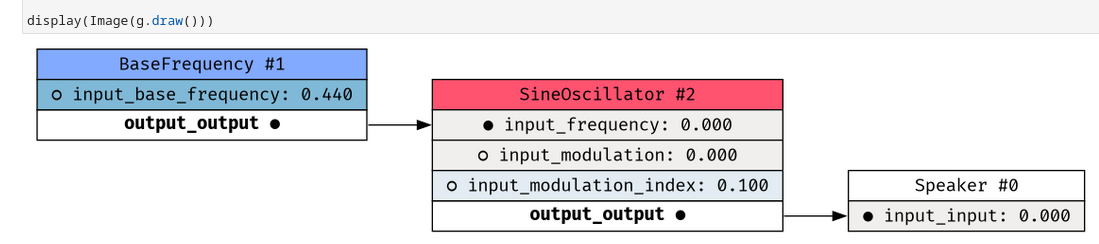
\includegraphics[width=1.0\linewidth]{rys02/simple_graph_creation_example.png}
    \caption{
      Wynik wykonania kodu przedstawionego w listingu~\ref{lst:simple_sine} w środowisku \textit{Jupyter Notebook},
      wizualizacja utworzonego grafu.
    }
    \label{fig:example_graph_creation_jupyter}
\end{figure}

\subsubsection{Uruchomienie procesu syntezy dźwięku}

Jak pokazano na listingu~\ref{lst:numpy_rust}, środowisko eksperymentalne zaimplementowane w ramach pracy w języku \texttt{Rust}
zwraca obiekty typu \texttt{ndarray}, wykorzystywane w większości pakietów obliczeniowych wykorzystywanych w języku \texttt{Python}.
Umożliwia to wykorzystanie gotowych bibliotek dostępnych w języku \texttt{Python},
aby przeanalizować sygnał lub zoptymalizować parametry syntezy \cite{2020SciPy-NMeth} \cite{librosa}.

\begin{lstlisting}[language=python, caption=Typ danych zwracanych przez środowisko eksperymentalne., label={lst:numpy_rust}]
>>> generated_signal = g.play(num_samples=100)
>>> type(generated_signal)
<class `numpy.ndarray'>
\end{lstlisting}

\subsection{Detale techniczne}

\subsubsection{Połączenia między węzłami w grafie}

Ponieważ wymagania zdefiniowane w rozdziale~\ref{sec:requirements} zawierają dynamiczne modyfikowanie grafu przetwarzania sygnałów,
nie jest możliwe spredefiniowanie mechanizmu wymiany danych między połączonymi węzłami.
Podczas implementacji rozważane były następujące architektury:

\begin{enumerate}
  \item Przejście przez graf przed uruchomieniem syntezy i określenie kolejności wywołania węzłów,
  \item Wykorzystanie struktury danych kolejki w każdym połączeniu,
  \item Bezpośrednie przepisywanie wartości wyjść z węzłów do modulowanych przez nie wejść po każdej iteracji przetwarzania. \label{test}
\end{enumerate}

Ostatecznie wybrane zostało podejście 3, ze względu na konieczność spełnienia wymagania~\ref{sec:modulation_requirements},
konkretnie możliwości modulowania wejścia danego węzła
przez wyjście tego samego węzła, co uniemożliwia wykorzystanie podejścia 1. Jednocześnie
podejście 3 jest łatwiejsze do implementacji niż podejście 2. Implementację mechanizmu
przesyłu danych między węzłami ułatwiło wykorzystanie makr proceduralnych, opisane w sekcji~\ref{sec:proc_macro}.

\subsubsection{Zastosowanie \textit{procedural macros} do automatycznej generacji akcesorów struktur węzłów} \label{sec:proc_macro}

% Przesyłanie wartości modulacji między węzłami grafu wymaga zdefiniowania struktur mapujących
% poszczególne pola struktur danych na ich indeksy, dzięki czemu możliwe jes
Podczas implementacji grafu DSP zostały wykorzystane makra proceduralne~\cite{proc_macro},
które umożliwiają automatyczne zaimplementowanie metod odczytujących $i$-te wejście
lub wyjście danego węzła. Alternatywnym podejściem byłoby wykorzystanie struktur takich
jak słowniki lub mapy, które umożliwiają na inspekcję kluczy w strukturze danych podczas
działania programu i dostęp do nich za pomocą indeksu, jednakże takie podejście zmniejsza
wydajność programu i nie wykorzystuje wykorzystywanie systemu typów wbudowanego w język,
co potencjalnie może być źródłem błędów podczas utrzymywania dużego zbioru węzłów i algorytmów,
które wykonują. Wykorzystanie makr proceduralnych pozwala na ograniczenie powtarzalnych
implementacji podobnych akcesorów i zachowanie zalet silnego systemu typów języka
\texttt{Rust}. % ponieważ na poziomie implementacji

\subsubsection{Implementacja natywnego modułu dla języka \texttt{Python}}

Aby umożliwić wykorzystanie grafu przetwarzania sygnałów z poziomu języka
Python, wykorzystano narzędzie \textit{Maturin}~\cite{maturin}, służące
do implementowania rozszerzeń zgodnych ze standardem \textit{Python Extension Module}~\cite{python_extension_module}
w języku \texttt{Rust}.

